\documentclass[twoside]{book}

% Packages required by doxygen
\usepackage{fixltx2e}
\usepackage{calc}
\usepackage{doxygen}
\usepackage[export]{adjustbox} % also loads graphicx
\usepackage{graphicx}
\usepackage[utf8]{inputenc}
\usepackage{makeidx}
\usepackage{multicol}
\usepackage{multirow}
\PassOptionsToPackage{warn}{textcomp}
\usepackage{textcomp}
\usepackage[nointegrals]{wasysym}
\usepackage[table]{xcolor}

% Font selection
\usepackage[T1]{fontenc}
\usepackage[scaled=.90]{helvet}
\usepackage{courier}
\usepackage{amssymb}
\usepackage{sectsty}
\renewcommand{\familydefault}{\sfdefault}
\allsectionsfont{%
  \fontseries{bc}\selectfont%
  \color{darkgray}%
}
\renewcommand{\DoxyLabelFont}{%
  \fontseries{bc}\selectfont%
  \color{darkgray}%
}
\newcommand{\+}{\discretionary{\mbox{\scriptsize$\hookleftarrow$}}{}{}}

% Page & text layout
\usepackage{geometry}
\geometry{%
  a4paper,%
  top=2.5cm,%
  bottom=2.5cm,%
  left=2.5cm,%
  right=2.5cm%
}
\tolerance=750
\hfuzz=15pt
\hbadness=750
\setlength{\emergencystretch}{15pt}
\setlength{\parindent}{0cm}
\setlength{\parskip}{3ex plus 2ex minus 2ex}
\makeatletter
\renewcommand{\paragraph}{%
  \@startsection{paragraph}{4}{0ex}{-1.0ex}{1.0ex}{%
    \normalfont\normalsize\bfseries\SS@parafont%
  }%
}
\renewcommand{\subparagraph}{%
  \@startsection{subparagraph}{5}{0ex}{-1.0ex}{1.0ex}{%
    \normalfont\normalsize\bfseries\SS@subparafont%
  }%
}
\makeatother

% Headers & footers
\usepackage{fancyhdr}
\pagestyle{fancyplain}
\fancyhead[LE]{\fancyplain{}{\bfseries\thepage}}
\fancyhead[CE]{\fancyplain{}{}}
\fancyhead[RE]{\fancyplain{}{\bfseries\leftmark}}
\fancyhead[LO]{\fancyplain{}{\bfseries\rightmark}}
\fancyhead[CO]{\fancyplain{}{}}
\fancyhead[RO]{\fancyplain{}{\bfseries\thepage}}
\fancyfoot[LE]{\fancyplain{}{}}
\fancyfoot[CE]{\fancyplain{}{}}
\fancyfoot[RE]{\fancyplain{}{\bfseries\scriptsize Generated by Doxygen }}
\fancyfoot[LO]{\fancyplain{}{\bfseries\scriptsize Generated by Doxygen }}
\fancyfoot[CO]{\fancyplain{}{}}
\fancyfoot[RO]{\fancyplain{}{}}
\renewcommand{\footrulewidth}{0.4pt}
\renewcommand{\chaptermark}[1]{%
  \markboth{#1}{}%
}
\renewcommand{\sectionmark}[1]{%
  \markright{\thesection\ #1}%
}

% Indices & bibliography
\usepackage{natbib}
\usepackage[titles]{tocloft}
\setcounter{tocdepth}{3}
\setcounter{secnumdepth}{5}
\makeindex

% Hyperlinks (required, but should be loaded last)
\usepackage{ifpdf}
\ifpdf
  \usepackage[pdftex,pagebackref=true]{hyperref}
\else
  \usepackage[ps2pdf,pagebackref=true]{hyperref}
\fi
\hypersetup{%
  colorlinks=true,%
  linkcolor=blue,%
  citecolor=blue,%
  unicode%
}

% Custom commands
\newcommand{\clearemptydoublepage}{%
  \newpage{\pagestyle{empty}\cleardoublepage}%
}

\usepackage{caption}
\captionsetup{labelsep=space,justification=centering,font={bf},singlelinecheck=off,skip=4pt,position=top}

%===== C O N T E N T S =====

\begin{document}

% Titlepage & ToC
\hypersetup{pageanchor=false,
             bookmarksnumbered=true,
             pdfencoding=unicode
            }
\pagenumbering{roman}
\begin{titlepage}
\vspace*{7cm}
\begin{center}%
{\Large My Project }\\
\vspace*{1cm}
{\large Generated by Doxygen 1.8.11}\\
\end{center}
\end{titlepage}
\clearemptydoublepage
\tableofcontents
\clearemptydoublepage
\pagenumbering{arabic}
\hypersetup{pageanchor=true}

%--- Begin generated contents ---
\chapter{Class Index}
\section{Class List}
Here are the classes, structs, unions and interfaces with brief descriptions\+:\begin{DoxyCompactList}
\item\contentsline{section}{\hyperlink{structg1_1_1package__block}{g1\+::package\+\_\+block} \\*Структура-\/описатель блока. Создается поверх пакета для упрощения работы с ним }{\pageref{structg1_1_1package__block}}{}
\item\contentsline{section}{\hyperlink{structg1_1_1package__header}{g1\+::package\+\_\+header} \\*Структура заголовок пакета }{\pageref{structg1_1_1package__header}}{}
\end{DoxyCompactList}

\chapter{File Index}
\section{File List}
Here is a list of all documented files with brief descriptions\+:\begin{DoxyCompactList}
\item\contentsline{section}{/home/mirmik/project/g1/g1/{\bfseries gateway.\+h} }{\pageref{gateway_8h}}{}
\item\contentsline{section}{/home/mirmik/project/g1/g1/{\bfseries indexes.\+h} }{\pageref{indexes_8h}}{}
\item\contentsline{section}{/home/mirmik/project/g1/g1/\hyperlink{packet_8h}{packet.\+h} \\*Всё, что касается работы с пакетом }{\pageref{packet_8h}}{}
\item\contentsline{section}{/home/mirmik/project/g1/g1/\hyperlink{tower_8h}{tower.\+h} \\*Tower file }{\pageref{tower_8h}}{}
\end{DoxyCompactList}

\chapter{Class Documentation}
\hypertarget{structg1_1_1package}{}\section{g1\+:\+:package Struct Reference}
\label{structg1_1_1package}\index{g1\+::package@{g1\+::package}}


Структура-\/описатель блока. Создается поверх пакета для упрощения работы с ним.  




{\ttfamily \#include $<$g1.\+h$>$}



Collaboration diagram for g1\+:\+:package\+:
\nopagebreak
\begin{figure}[H]
\begin{center}
\leavevmode
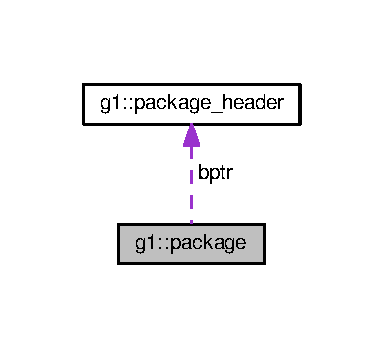
\includegraphics[width=184pt]{structg1_1_1package__coll__graph}
\end{center}
\end{figure}
\subsection*{Public Member Functions}
\begin{DoxyCompactItemize}
\item 
void \hyperlink{structg1_1_1package_a667ed03d442d2c9cfe28917c75525e4e}{revert\+\_\+stage} (uint8\+\_\+t size, void $\ast$addr)
\end{DoxyCompactItemize}
\subsection*{Public Attributes}
\begin{DoxyCompactItemize}
\item 
\hyperlink{structg1_1_1package__header}{package\+\_\+header} $\ast$ \hyperlink{structg1_1_1package_a1e75b5ccd00f3b8bd3c7958bc6d957e9}{bptr}\hypertarget{structg1_1_1package_a1e75b5ccd00f3b8bd3c7958bc6d957e9}{}\label{structg1_1_1package_a1e75b5ccd00f3b8bd3c7958bc6d957e9}

\begin{DoxyCompactList}\small\item\em Указатель на заголовок реферируемого блока \end{DoxyCompactList}\end{DoxyCompactItemize}


\subsection{Detailed Description}
Структура-\/описатель блока. Создается поверх пакета для упрощения работы с ним. 

\subsection{Member Function Documentation}
\index{g1\+::package@{g1\+::package}!revert\+\_\+stage@{revert\+\_\+stage}}
\index{revert\+\_\+stage@{revert\+\_\+stage}!g1\+::package@{g1\+::package}}
\subsubsection[{\texorpdfstring{revert\+\_\+stage(uint8\+\_\+t size, void $\ast$addr)}{revert_stage(uint8_t size, void *addr)}}]{\setlength{\rightskip}{0pt plus 5cm}void g1\+::package\+::revert\+\_\+stage (
\begin{DoxyParamCaption}
\item[{uint8\+\_\+t}]{size, }
\item[{void $\ast$}]{addr}
\end{DoxyParamCaption}
)}\hypertarget{structg1_1_1package_a667ed03d442d2c9cfe28917c75525e4e}{}\label{structg1_1_1package_a667ed03d442d2c9cfe28917c75525e4e}
Отметить в пакете прохождение врат. 

The documentation for this struct was generated from the following file\+:\begin{DoxyCompactItemize}
\item 
/home/rfmeas/project/g1/g1/\hyperlink{g1_8h}{g1.\+h}\end{DoxyCompactItemize}

\hypertarget{structg1_1_1package__header}{}\section{g1\+:\+:package\+\_\+header Struct Reference}
\label{structg1_1_1package__header}\index{g1\+::package\+\_\+header@{g1\+::package\+\_\+header}}


Структура заголовок пакета.  




{\ttfamily \#include $<$g1.\+h$>$}

\subsection*{Public Attributes}
\begin{DoxyCompactItemize}
\item 
uint8\+\_\+t \hyperlink{structg1_1_1package__header_a77aeda3b76d39b1067afd494c58873af}{type}\hypertarget{structg1_1_1package__header_a77aeda3b76d39b1067afd494c58873af}{}\label{structg1_1_1package__header_a77aeda3b76d39b1067afd494c58873af}

\begin{DoxyCompactList}\small\item\em Тип \end{DoxyCompactList}\item 
uint16\+\_\+t {\bfseries flen}\hypertarget{structg1_1_1package__header_a148b733fe97c06f0ded129f2a1d953c1}{}\label{structg1_1_1package__header_a148b733fe97c06f0ded129f2a1d953c1}

\item 
uint16\+\_\+t {\bfseries seqid}\hypertarget{structg1_1_1package__header_a8f706d30ff3d9154aff97827aa291af8}{}\label{structg1_1_1package__header_a8f706d30ff3d9154aff97827aa291af8}

\item 
uint8\+\_\+t {\bfseries alen}\hypertarget{structg1_1_1package__header_aca2dc89b824e81d9aaa99488aab21fe7}{}\label{structg1_1_1package__header_aca2dc89b824e81d9aaa99488aab21fe7}

\item 
uint8\+\_\+t {\bfseries stg}\hypertarget{structg1_1_1package__header_ade59c95e617ca8789a408c9aaa0ab088}{}\label{structg1_1_1package__header_ade59c95e617ca8789a408c9aaa0ab088}

\item 
\hyperlink{g1_8h_a157fb77f1b8142697dc1b88efaae6a0a}{QoS} {\bfseries qos}\hypertarget{structg1_1_1package__header_aea47ad75b2af7d91d1f460ff5887c751}{}\label{structg1_1_1package__header_aea47ad75b2af7d91d1f460ff5887c751}

\end{DoxyCompactItemize}


\subsection{Detailed Description}
Структура заголовок пакета. 

The documentation for this struct was generated from the following file\+:\begin{DoxyCompactItemize}
\item 
/home/rfmeas/project/g1/g1/\hyperlink{g1_8h}{g1.\+h}\end{DoxyCompactItemize}

\chapter{File Documentation}
\hypertarget{g1_8h}{}\section{/home/mirmik/project/g1/g1/g1.h File Reference}
\label{g1_8h}\index{/home/mirmik/project/g1/g1/g1.\+h@{/home/mirmik/project/g1/g1/g1.\+h}}


G1 main file.  


{\ttfamily \#include $<$cstdint$>$}\\*
Include dependency graph for g1.\+h\+:\nopagebreak
\begin{figure}[H]
\begin{center}
\leavevmode
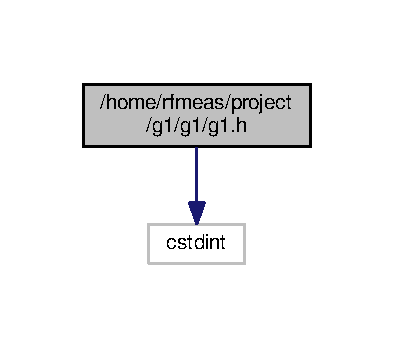
\includegraphics[width=189pt]{g1_8h__incl}
\end{center}
\end{figure}
\subsection*{Classes}
\begin{DoxyCompactItemize}
\item 
struct \hyperlink{structg1_1_1package__header}{g1\+::package\+\_\+header}
\begin{DoxyCompactList}\small\item\em Структура заголовок пакета. \end{DoxyCompactList}\item 
struct \hyperlink{structg1_1_1package}{g1\+::package}
\begin{DoxyCompactList}\small\item\em Структура-\/описатель блока. Создается поверх пакета для упрощения работы с ним. \end{DoxyCompactList}\end{DoxyCompactItemize}
\subsection*{Enumerations}
\begin{DoxyCompactItemize}
\item 
enum \hyperlink{g1_8h_a157fb77f1b8142697dc1b88efaae6a0a}{g1\+::\+QoS} \+: uint8\+\_\+t \{ \\*
\hyperlink{g1_8h_a157fb77f1b8142697dc1b88efaae6a0aac54b983a21cb9cc3e8ad8251daefa6eb}{g1\+::\+One}, 
\hyperlink{g1_8h_a157fb77f1b8142697dc1b88efaae6a0aa994c57f974d40a6ecc7422ba603d9cc2}{g1\+::\+Two}, 
\hyperlink{g1_8h_a157fb77f1b8142697dc1b88efaae6a0aa8c29c9985b72e9606b061e974c72ff34}{g1\+::\+Three}, 
\hyperlink{g1_8h_a157fb77f1b8142697dc1b88efaae6a0aac54b983a21cb9cc3e8ad8251daefa6eb}{g1\+::\+One}, 
\\*
\hyperlink{g1_8h_a157fb77f1b8142697dc1b88efaae6a0aa994c57f974d40a6ecc7422ba603d9cc2}{g1\+::\+Two}, 
\hyperlink{g1_8h_a157fb77f1b8142697dc1b88efaae6a0aa8c29c9985b72e9606b061e974c72ff34}{g1\+::\+Three}
 \}\begin{DoxyCompactList}\small\item\em Качество обслуживания. \end{DoxyCompactList}
\end{DoxyCompactItemize}
\subsection*{Functions}
\begin{DoxyCompactItemize}
\item 
void \hyperlink{g1_8h_a45e9a9c10b72eb4105e9521d506a2919}{g1\+::transport} (package pack)\hypertarget{g1_8h_a45e9a9c10b72eb4105e9521d506a2919}{}\label{g1_8h_a45e9a9c10b72eb4105e9521d506a2919}

\begin{DoxyCompactList}\small\item\em Переместить пакет дальше по конвееру врат. \end{DoxyCompactList}\end{DoxyCompactItemize}


\subsection{Detailed Description}
G1 main file. 



\subsection{Enumeration Type Documentation}
\index{g1.\+h@{g1.\+h}!QoS@{QoS}}
\index{QoS@{QoS}!g1.\+h@{g1.\+h}}
\subsubsection[{\texorpdfstring{QoS}{QoS}}]{\setlength{\rightskip}{0pt plus 5cm}enum {\bf g1\+::\+QoS} \+: uint8\+\_\+t}\hypertarget{g1_8h_file_a157fb77f1b8142697dc1b88efaae6a0a}{}\label{g1_8h_file_a157fb77f1b8142697dc1b88efaae6a0a}


Качество обслуживания. 

\begin{Desc}
\item[Enumerator]\par
\begin{description}
\index{One@{One}!g1.\+h@{g1.\+h}}\index{g1.\+h@{g1.\+h}!One@{One}}\item[{\em 
One\hypertarget{g1_8h_a157fb77f1b8142697dc1b88efaae6a0aac54b983a21cb9cc3e8ad8251daefa6eb}{}\label{g1_8h_a157fb77f1b8142697dc1b88efaae6a0aac54b983a21cb9cc3e8ad8251daefa6eb}
}]one \index{Two@{Two}!g1.\+h@{g1.\+h}}\index{g1.\+h@{g1.\+h}!Two@{Two}}\item[{\em 
Two\hypertarget{g1_8h_a157fb77f1b8142697dc1b88efaae6a0aa994c57f974d40a6ecc7422ba603d9cc2}{}\label{g1_8h_a157fb77f1b8142697dc1b88efaae6a0aa994c57f974d40a6ecc7422ba603d9cc2}
}]two \index{Three@{Three}!g1.\+h@{g1.\+h}}\index{g1.\+h@{g1.\+h}!Three@{Three}}\item[{\em 
Three\hypertarget{g1_8h_a157fb77f1b8142697dc1b88efaae6a0aa8c29c9985b72e9606b061e974c72ff34}{}\label{g1_8h_a157fb77f1b8142697dc1b88efaae6a0aa8c29c9985b72e9606b061e974c72ff34}
}]three \index{One@{One}!g1.\+h@{g1.\+h}}\index{g1.\+h@{g1.\+h}!One@{One}}\item[{\em 
One\hypertarget{g1_8h_a157fb77f1b8142697dc1b88efaae6a0aac54b983a21cb9cc3e8ad8251daefa6eb}{}\label{g1_8h_a157fb77f1b8142697dc1b88efaae6a0aac54b983a21cb9cc3e8ad8251daefa6eb}
}]one \index{Two@{Two}!g1.\+h@{g1.\+h}}\index{g1.\+h@{g1.\+h}!Two@{Two}}\item[{\em 
Two\hypertarget{g1_8h_a157fb77f1b8142697dc1b88efaae6a0aa994c57f974d40a6ecc7422ba603d9cc2}{}\label{g1_8h_a157fb77f1b8142697dc1b88efaae6a0aa994c57f974d40a6ecc7422ba603d9cc2}
}]two \index{Three@{Three}!g1.\+h@{g1.\+h}}\index{g1.\+h@{g1.\+h}!Three@{Three}}\item[{\em 
Three\hypertarget{g1_8h_a157fb77f1b8142697dc1b88efaae6a0aa8c29c9985b72e9606b061e974c72ff34}{}\label{g1_8h_a157fb77f1b8142697dc1b88efaae6a0aa8c29c9985b72e9606b061e974c72ff34}
}]three \end{description}
\end{Desc}

%--- End generated contents ---

% Index
\backmatter
\newpage
\phantomsection
\clearemptydoublepage
\addcontentsline{toc}{chapter}{Index}
\printindex

\end{document}
